
\appendix

\chapter{Mã nguồn một số phương thức quan trọng}

Phụ lục này trình bày một số phương thức tiêu biểu trong mã nguồn của hệ thống, được lựa chọn dựa trên mức độ quan trọng trong việc minh họa kiến trúc hệ thống và giải quyết các yêu cầu nghiệp vụ. Các API này không chỉ thực hiện các thao tác CRUD cơ bản mà còn bao hàm các thuật toán xử lý dữ liệu, cơ chế học tập theo \textit{spaced repetition}, cũng như yếu tố \textit{gamification} thông qua hệ thống thú cưng. 

Mục tiêu của phụ lục là cung cấp cho người đọc cái nhìn rõ ràng về cách hiện thực hoá các yêu cầu chức năng, thay vì liệt kê toàn bộ mã nguồn.

\section{API Quản lý Phiên Học}

\textbf{Mục đích:} Khởi tạo, quản lý và hoàn tất các phiên học hoặc ôn tập của người dùng. Đây là điểm vào (entry point) chính để bắt đầu luồng học.

\begin{lstlisting}[language=C, caption={Tạo một phiên học dựa trên bộ từ vựng đã chọn}]
[Authorize(Roles = "User")]
[HttpPost("{vocaSetId}")]
public async Task<IActionResult> CreateLearningSession(int vocaSetId)
{
    var userId = User.GetUserId();
    if (userId == 0) return Unauthorized();
    if (vocaSetId <= 0) return BadRequest("Invalid VocabularySet ID");

    try
    {
        var learningSessionDto = await _learningSessionService.CreateLearningSessionAsync(userId, vocaSetId);
        return Ok(learningSessionDto);
    }
    catch (InvalidOperationException ex)
    {
        _logger.LogWarning(ex, "No unlearned vocabularies found.");
        return NotFound(ex.Message);
    }
}
\end{lstlisting}

API trên thể hiện rõ cách hệ thống:
\begin{itemize}
    \item Xác thực người dùng thông qua JWT và Role.
    \item Kiểm tra quyền sở hữu bộ từ vựng.
    \item Xử lý tình huống không còn từ để học và trả về mã lỗi phù hợp.
\end{itemize}

\section{Thuật Toán Cập Nhật Tiến Trình Học }

\textbf{Mục đích:} Lưu kết quả trả lời và áp dụng cơ chế \textit{spaced repetition} để xác định thời điểm ôn tập tiếp theo.

\begin{lstlisting}[language=C, caption={Cập nhật tiến trình học và tính ngày ôn tập}]
progress.ProficiencyLevel = Math.Min(5, 
    1 + (int)Math.Floor(Math.Log(Math.Max(1, progress.CorrectAttempt), 1.5)));

int daysToAdd = progress.ProficiencyLevel switch
{
    1 => 1,
    2 => 2,
    3 => 4,
    4 => 16,
    _ => 256
};

progress.NextReviewTime = DateTime.UtcNow.AddDays(daysToAdd);
\end{lstlisting}

Đây là phần mang tính học thuật quan trọng, vì nó giúp hệ thống tối ưu tần suất xuất hiện của từ vựng, đảm bảo người học ghi nhớ lâu hơn mà không quá tải.

\section{API Tạo Bộ Từ Vựng }

\textbf{Mục đích:} Tạo bộ từ vựng mới và tự động gán thú cưng phần thưởng theo độ hiếm.

\begin{lstlisting}[language=C, caption={Tự động gán Pet thưởng cho bộ từ vựng}]
var petDistribution = new Dictionary<PetRarity, (int Count, double DropRate)>
{
    { PetRarity.Common, (10, 0.4) },
    { PetRarity.Uncommon, (5, 0.25) },
    { PetRarity.Rare, (3, 0.15) },
    { PetRarity.Epic, (2, 0.05) },
    { PetRarity.Legendary, (1, 0.01) }
};

foreach (var (rarity, (count, dropRate)) in petDistribution)
{
    var pets = await _petRepository.GetRandomPetsByRarityAsync(rarity, count);
    vocabularySet.SetRewardPets.AddRange(pets.Select(pet => new SetRewardPet
    {
        PetId = pet.Id,
        DropRate = dropRate
    }));
}
\end{lstlisting}

Đoạn mã này cho thấy cách hệ thống sử dụng logic xác suất để phân phối phần thưởng, góp phần tăng tính hấp dẫn của quá trình học.

\section{API Nâng Cấp Thú Cưng}

\textbf{Mục đích:} Xử lý logic tăng kinh nghiệm, tăng cấp độ và tiến hoá thú cưng, từ đó gắn kết yếu tố trò chơi vào hệ thống học.

\begin{lstlisting}[language=C, caption={Nâng cấp và tiến hóa thú cưng}]
while (userOwnedPet.Experience >= 100)
{
    userOwnedPet.Level++;
    userOwnedPet.Experience -= 100;
    isLevelUp = true;

    if (currentPet.RequiredLevel != null && 
        userOwnedPet.Level >= currentPet.RequiredLevel &&
        currentPet.NextEvolutionId.HasValue)
    {
        var evolvedPet = await _petRepository.GetPetByIdAsync(currentPet.NextEvolutionId.Value);
        if (evolvedPet != null)
        {
            userOwnedPet.PetId = evolvedPet.Id;
            isEvolve = true;
            break;
        }
    }
}
\end{lstlisting}

API này minh họa cách hệ thống quản lý trạng thái phức tạp của thú cưng, đồng thời đảm bảo tính nhất quán dữ liệu khi người dùng nâng cấp nhiều lần liên tiếp.

\section{Nhận Xét Chung}

Các API trên thể hiện:
\begin{itemize}
    \item Cách hệ thống kết hợp giữa \textbf{xác thực – xử lý nghiệp vụ – lưu trữ dữ liệu}.
    \item Việc áp dụng thuật toán học tập và gamification.
    \item Thiết kế chuẩn RESTful, tách biệt Controller – Service – Repository, dễ mở rộng trong tương lai.
\end{itemize}

Các API CRUD cơ bản khác (xem/xoá/cập nhật Pet, tìm kiếm bộ từ vựng, quản lý người dùng) không được liệt kê ở đây để tránh trùng lặp và giữ tính cô đọng cho phụ lục.


\chapter{Một Số Màn Hình Bổ Sung}

Phụ lục này giới thiệu thêm một số màn hình giao diện của hệ thống , minh hoạ các chức năng phụ trợ như lọc, tìm kiếm, xem chi tiết và điều hướng học tập. Các màn hình này không được mô tả chi tiết trong chương Kết quả đạt được nhưng đóng vai trò quan trọng trong việc nâng cao trải nghiệm người dùng.

\section{Màn hình Danh sách Thú cưng}
\begin{figure}[H]
\centering
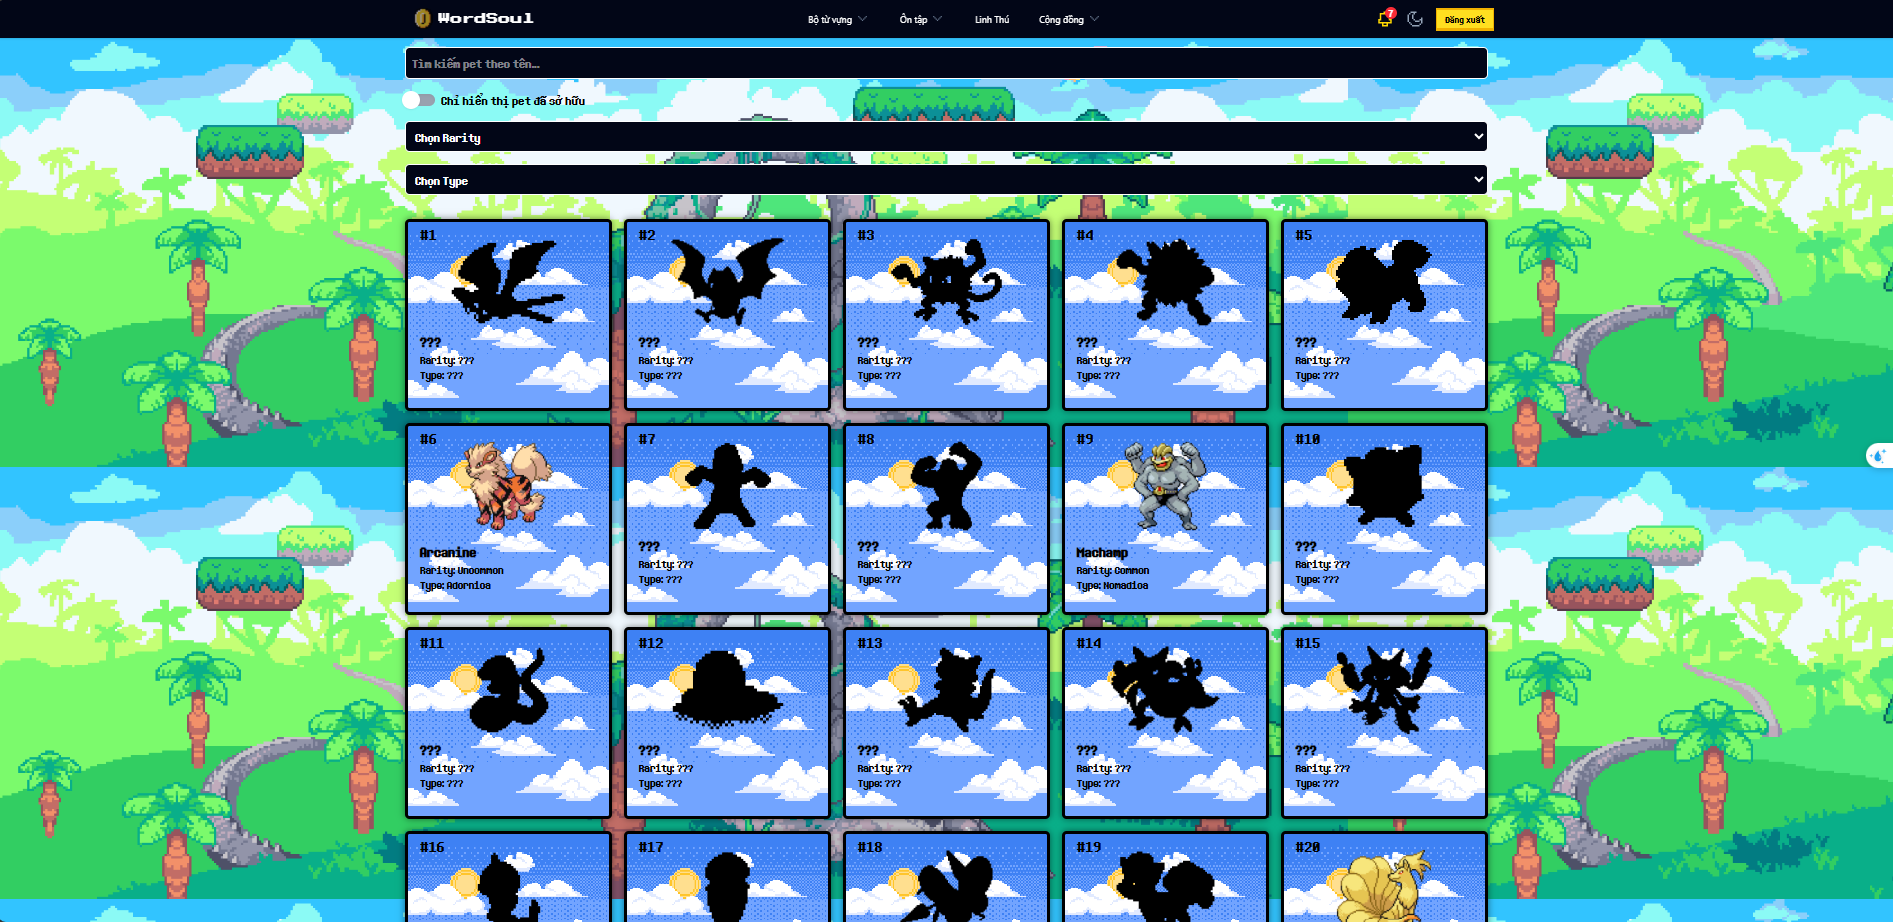
\includegraphics[width=15cm]{images/IF_PetList.png}
\caption{Màn hình danh sách thú cưng với bộ lọc nâng cao.}
\label{fig_pet_list}
\end{figure}

Màn hình này hiển thị toàn bộ thú cưng trong hệ thống và hỗ trợ:
\begin{itemize}
    \item Lọc theo tên thú cưng hoặc chỉ hiển thị thú đã sở hữu.
    \item Lọc theo độ hiếm (\textit{Common, Rare, Epic, Legendary}) và loại (\textit{Beast, Spirit, Machine,...}).
    \item Hiển thị trực quan tình trạng sở hữu, cấp độ hiện tại và tiến trình tiến hoá.
\end{itemize}
Chức năng này giúp người học dễ dàng theo dõi bộ sưu tập, tăng động lực thu thập đầy đủ thú cưng.

\section{Màn hình Chi tiết Bộ từ vựng}
\begin{figure}[H]
\centering
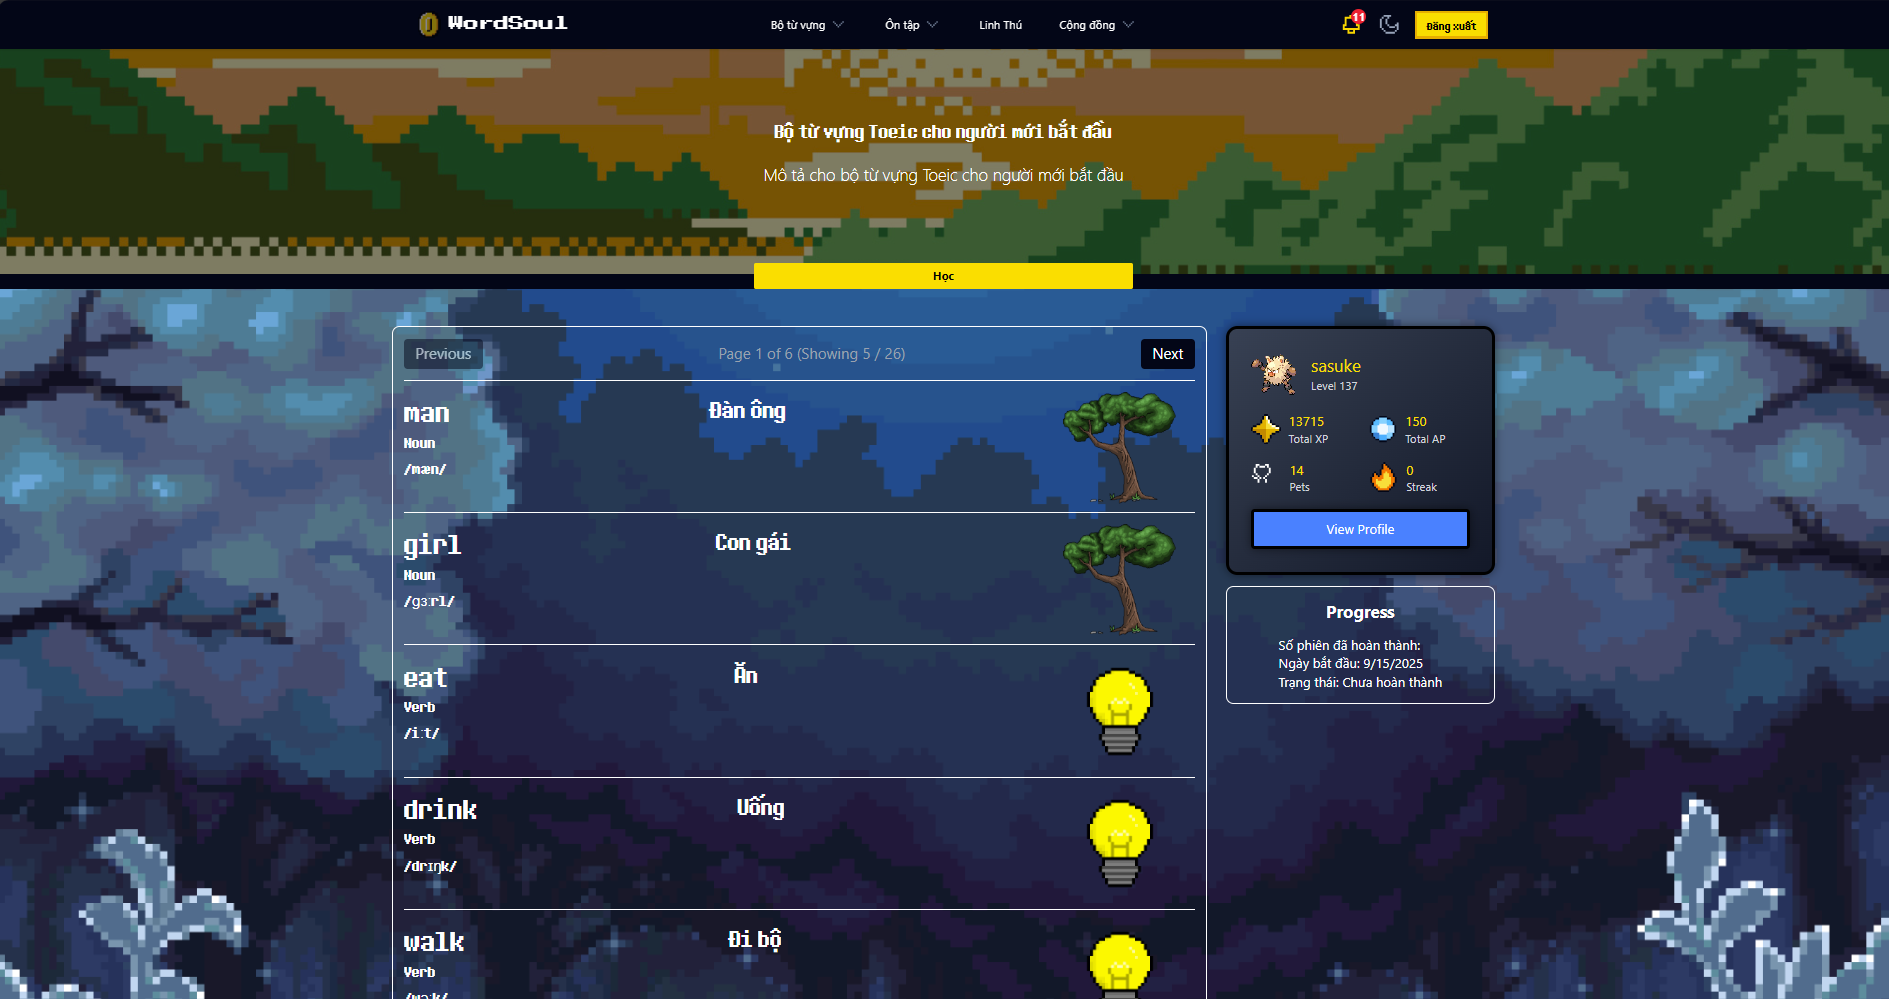
\includegraphics[width=15cm]{images/IF_SetDetail.png}
\caption{Màn hình chi tiết bộ từ vựng.}
\label{fig_set_detail}
\end{figure}

Màn hình này cung cấp thông tin toàn diện về một bộ từ:
\begin{itemize}
    \item Hiển thị tiêu đề, mô tả, ảnh minh họa, chủ đề, độ khó và thú cưng thưởng.
    \item Nút \textbf{Đăng ký bộ từ vựng} (nếu người dùng chưa sở hữu) và nút \textbf{Học} (nếu đã sở hữu).
    \item Nút \textbf{Đã hoàn thành} được disable khi người dùng đã học xong toàn bộ bộ từ.
    \item Danh sách tất cả các từ trong bộ, kèm tiến trình (ví dụ: số lần đúng, mức độ thành thạo).
\end{itemize}
Màn hình này là trung tâm định hướng học tập, giúp người dùng quyết định đăng ký hoặc tiếp tục học.

\section{Màn hình Danh sách Bộ từ vựng}
\begin{figure}[H]
\centering
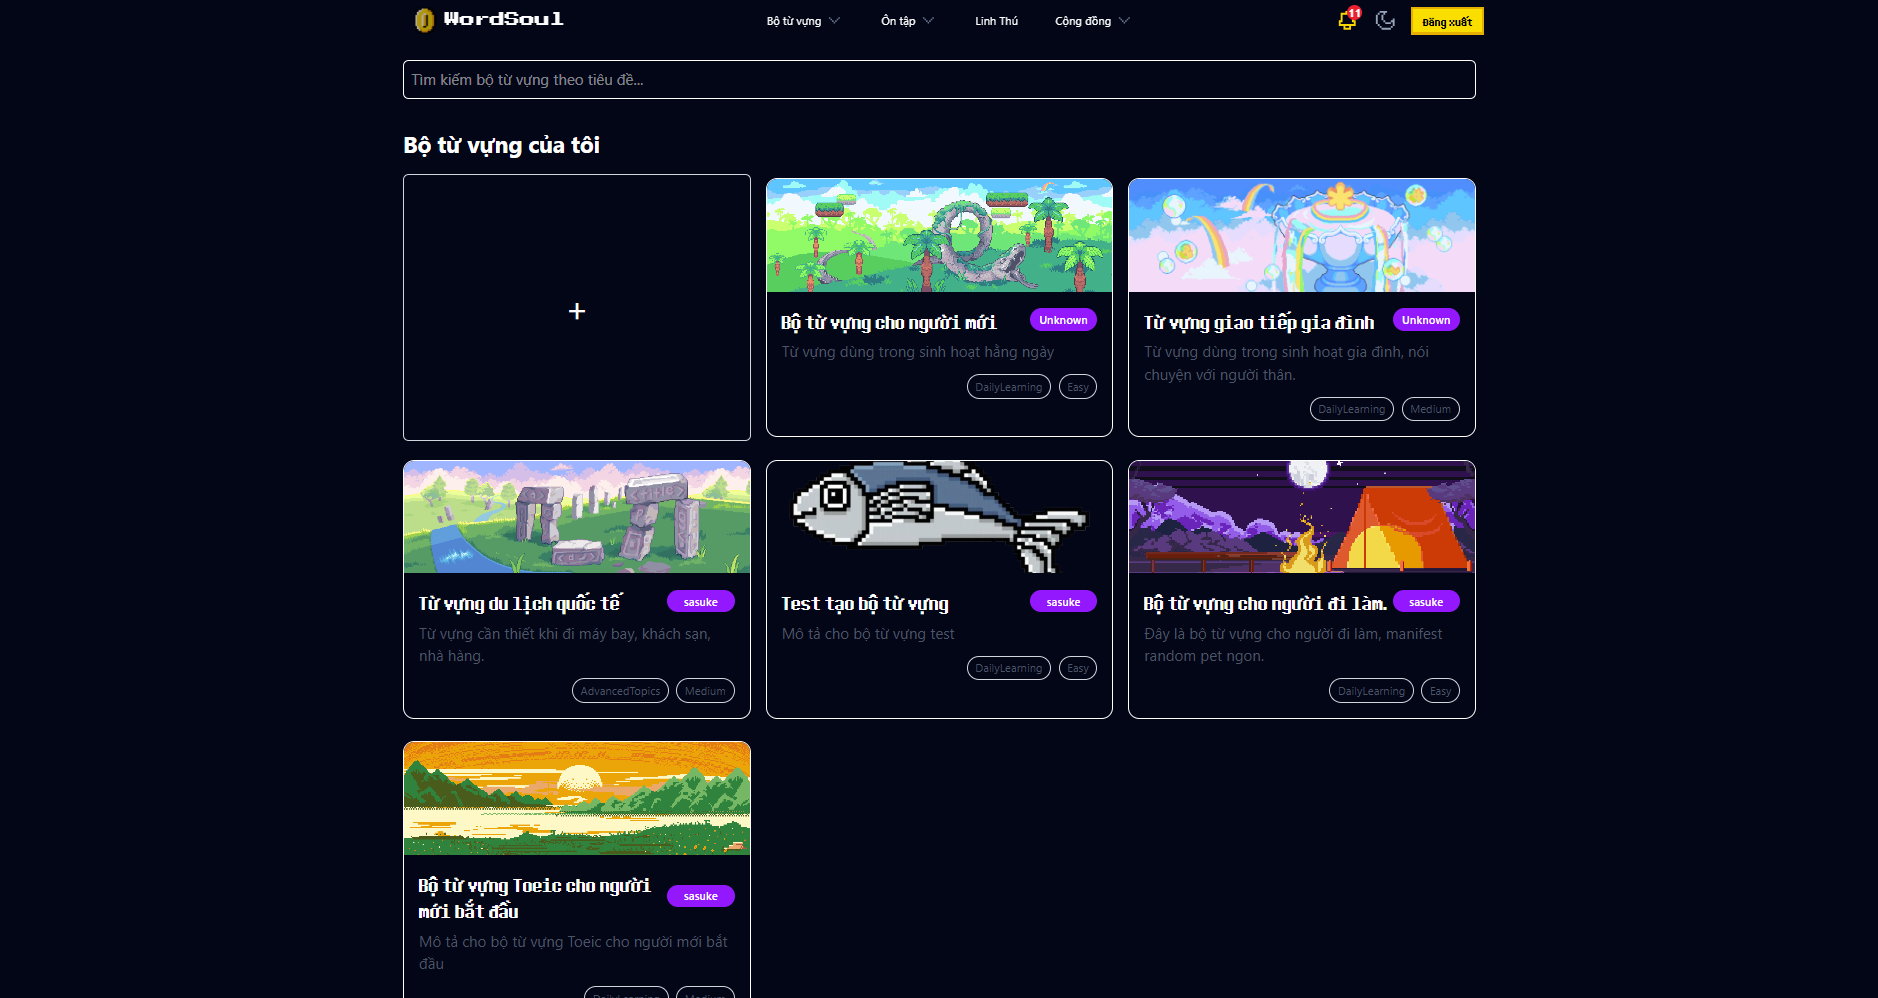
\includegraphics[width=15cm]{images/IF_SetList.png}
\caption{Màn hình danh sách bộ từ vựng.}
\label{fig_set_list}
\end{figure}

Màn hình này cho phép duyệt và tìm kiếm bộ từ vựng:
\begin{itemize}
    \item Lọc theo \textbf{chủ đề} (Theme) và mức độ khó.
    \item Tìm kiếm theo từ khóa để nhanh chóng tìm bộ từ liên quan.
    \item Hiển thị trạng thái sở hữu và số lượng từ còn phải học trong từng bộ.
\end{itemize}

\section{Ý nghĩa và Vai trò}
Các màn hình trong phụ lục này thể hiện sự quan tâm đến \textbf{trải nghiệm người dùng (UX)}:
\begin{itemize}
    \item Tối ưu quá trình điều hướng: người học dễ tìm bộ từ, chọn pet hoặc kiểm tra tiến trình.
    \item Tăng tính cá nhân hóa: hiển thị rõ tình trạng sở hữu, tiến trình học, và khuyến khích hoàn thành.
    \item Hỗ trợ việc mở rộng sau này: thêm bộ lọc nâng cao, sắp xếp theo mức độ phổ biến hoặc ngày tạo.
\end{itemize}
Những màn hình này đóng vai trò quan trọng trong việc biến hệ thống thành một nền tảng học tập có tính cộng đồng và khuyến khích người học quay lại hằng ngày.
